% Vietnamese translation for OI Public Library
% Source-PDF: 动态规划 DYNAMIC PROGRAMMING/动态规划之四边形不等式优化 - 贺洪鸣.pdf
\documentclass[11pt]{article}
\usepackage{oipl-vn}
\usepackage{tikz}
\usetikzlibrary{arrows.meta}
\renewcommand{\figurename}{Hình}

\title{Tối ưu quy hoạch động bằng bất đẳng thức tứ giác}
\author{He Hongming}
\date{}

\begin{document}
\maketitle

\origtitle{Quadrangle Inequality Optimization in Dynamic Programming}
\sourcepath{Dynamic Programming / Quadrangle Inequality Optimization - He Hongming.pdf}

\section*{Bất đẳng thức tứ giác}

Với $a\le b\le c\le d$, nếu $w[a,c]+w[b,d]$ không kém hơn
$w[a,d]+w[b,c]$, ta nói $w$ thỏa mãn \term{bất đẳng thức tứ giác}.

Ở đây ``không kém hơn'' được hiểu theo hướng tối ưu của bài toán:
\begin{enumerate}
  \item Với bài toán tìm giá trị nhỏ nhất:
  \[
    w[a,c]+w[b,d]\le w[a,d]+w[b,c].
  \]
  \item Với bài toán tìm giá trị lớn nhất:
  \[
    w[a,c]+w[b,d]\ge w[a,d]+w[b,c].
  \]
\end{enumerate}

\section*{Tính đơn điệu theo bao hàm đoạn}

Nếu $[a,b]\subseteq[c,d]$ thì
\[
  w[a,b]\le w[c,d].
\]

Trực quan, trên bốn điểm theo thứ tự $a,b,c,d$, đại lượng
$w[a,c]+w[b,d]$ tốt hơn $w[a,d]+w[b,c]$ có thể được nhìn như việc so sánh
hai cách ghép các đoạn trên một tứ giác. Với bài toán cực tiểu, ``tốt hơn''
nghĩa là không lớn hơn; với bài toán cực đại, nghĩa là không nhỏ hơn.

\begin{figure}[ht]
\centering
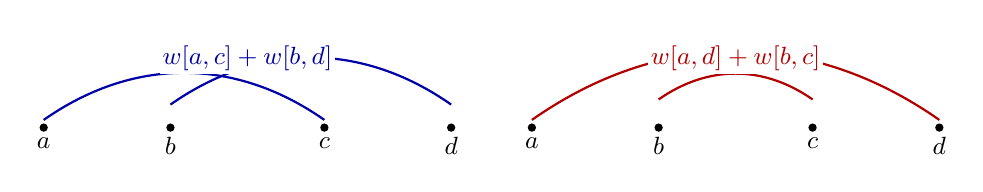
\begin{tikzpicture}[x=1.15cm,y=.65cm,>=Stealth,font=\small]
  \foreach \x/\lab in {0/a,1.4/b,3.1/c,4.5/d} {
    \fill (\x,0) circle (1.5pt);
    \node[below] at (\x,0) {$\lab$};
  }
  \draw[blue!65!black,thick] (0,.15) to[bend left=35] (3.1,.15);
  \draw[blue!65!black,thick] (1.4,.45) to[bend left=35] (4.5,.45);
  \node[blue!65!black,fill=white,inner sep=1pt] at (2.25,1.35) {$w[a,c]+w[b,d]$};

  \begin{scope}[xshift=6.2cm]
    \foreach \x/\lab in {0/a,1.4/b,3.1/c,4.5/d} {
      \fill (\x,0) circle (1.5pt);
      \node[below] at (\x,0) {$\lab$};
    }
    \draw[red!70!black,thick] (0,.15) to[bend left=35] (4.5,.15);
    \draw[red!70!black,thick] (1.4,.55) to[bend left=35] (3.1,.55);
    \node[red!70!black,fill=white,inner sep=1pt] at (2.25,1.35) {$w[a,d]+w[b,c]$};
  \end{scope}
\end{tikzpicture}
\caption{Hai cách ghép đoạn trong cách nhìn trực quan của bất đẳng thức tứ giác.}
\end{figure}

\section{Ví dụ 1: Gộp đá}

Bài NOI 1995.

\subsection*{Đề bài}

Trên một sân có một hàng gồm $n$ đống đá, $1\le n\le 1000$. Cần gộp các đống
đá theo thứ tự thành một đống duy nhất. Mỗi lần chỉ được chọn hai đống kề
nhau để gộp thành một đống mới, và số viên đá của đống mới được tính là điểm
của lần gộp đó.

Hãy tìm tổng điểm nhỏ nhất và lớn nhất để gộp $n$ đống đá thành một đống. Số
đá trong mỗi đống ban đầu là một số nguyên dương từ $1$ đến $1000$.

\subsection*{Phân tích sơ bộ}

Ta xét bài toán tìm tổng điểm nhỏ nhất; với tổng điểm lớn nhất chỉ cần đổi
hướng tối ưu từ $\min$ sang $\max$.

Định nghĩa trạng thái:
\begin{enumerate}
  \item $w[i,j]$ là tổng số đá từ đống $i$ đến đống $j$.
  \item $f[i,j]$ là tổng điểm nhỏ nhất để gộp các đống từ $i$ đến $j$ thành
  một đống.
  \item Đáp án cần tìm là $f[1,n]$.
\end{enumerate}

Phương trình chuyển trạng thái là
\[
  f[i,j]=\min_{i+1\le k\le j}
    \{f[i,k-1]+f[k,j]+w[i,j]\},
  \qquad f[i,i]=0,\ 1\le i\le n.
\]

Có $O(n^2)$ trạng thái, mỗi trạng thái có $O(n)$ quyết định, nên độ phức tạp
thời gian là $O(n^3)$.

Ký hiệu $k=s[i,j]$ là quyết định lớn nhất làm cho $f[i,j]$ đạt giá trị tối
ưu. Tức là
\[
  f[i,j]=f[i,k-1]+f[k,j]+w[i,j],
\]
và:
\begin{enumerate}
  \item nếu $p<k$ thì
  \[
    f[i,p-1]+f[p,j]+w[i,j]\ge f[i,k-1]+f[k,j]+w[i,j];
  \]
  \item nếu $p>k$ thì
  \[
    f[i,p-1]+f[p,j]+w[i,j]>f[i,k-1]+f[k,j]+w[i,j].
  \]
\end{enumerate}

\paragraph{Định lý 1.}
Với mọi số nguyên $a\le b\le c\le d$, nếu hàm $w$ thỏa mãn bất đẳng thức tứ
giác
\[
  w[a,c]+w[b,d]\le w[a,d]+w[b,c],
\]
thì hàm $f$ cũng thỏa mãn bất đẳng thức tứ giác:
\[
  f[a,c]+f[b,d]\le f[a,d]+f[b,c].
\]

\paragraph{Định lý 2.}
Với mọi số nguyên dương $a,b,c,d$ thỏa mãn $a\le b\le c\le d$, nếu hàm $f$
thỏa mãn bất đẳng thức tứ giác
\[
  f[a,c]+f[b,d]\le f[a,d]+f[b,c],
\]
thì quyết định $s[i,j]$ đơn điệu không giảm theo cả $i$ và $j$:
\[
  s[i,j-1]\le s[i,j]\le s[i+1,j].
\]

Trong ví dụ này, hàm $w$ hiển nhiên thỏa mãn bất đẳng thức tứ giác; thực ra
\[
  w[a,c]+w[b,d]=w[a,d]+w[b,c].
\]
Vì vậy, nếu Định lý 1 và Định lý 2 đúng, thì quyết định $s[i,j]$ đơn điệu
không giảm theo cả $i$ và $j$. Chứng minh của hai định lý được trình bày ở
phần sau.

\paragraph{Hệ quả 1.}
Với tất cả các trạng thái dạng $f[i,i+L]$, $1\le i\le n-L$, tổng số quyết
định cần xét không vượt quá $n$.

\paragraph{Chứng minh.}
Khi tính $f[i,j]$, khoảng giá trị của quyết định $k$ là
\[
  [s[i,j-1],s[i+1,j]].
\]
Do đó, với các trạng thái có cùng độ dài $L+1$, số quyết định lần lượt là
\[
\begin{aligned}
  &s[2,L+1]-s[1,L],\\
  &s[3,L+2]-s[2,L+1],\\
  &s[4,L+3]-s[3,L+2],\\
  &\cdots\\
  &s[n-L+1,n]-s[n-L,n-1].
\end{aligned}
\]
Tổng các giá trị này triệt tiêu kiểu dây chuyền, còn lại
\[
  s[n-L+1,n]-s[1,L]<s[n-L+1,n]\le n.
\]
Hệ quả được chứng minh.

\paragraph{Hệ quả 2.}
Nếu quyết định $s[i,j]$ đơn điệu không giảm theo $i$ và $j$, thì Ví dụ 1 có
thể giải trong thời gian $O(n^2)$.

\paragraph{Chứng minh.}
Theo Hệ quả 1, với mỗi $L=1,\ldots,n-1$, tổng số quyết định cần xét là
$O(n)$. Cộng trên mọi $L$, ta được thời gian $O(n^2)$.

\subsection*{Chứng minh Định lý 1}

Ta chứng minh: với mọi số nguyên dương $a,b,c,d$ thỏa mãn
$a\le b\le c\le d$, nếu
\[
  w[a,c]+w[b,d]\le w[a,d]+w[b,c],
\]
thì
\[
  f[a,c]+f[b,d]\le f[a,d]+f[b,c].
\]

\begin{enumerate}
  \item Nếu $a=b$, thì
  \[
    f[a,c]+f[b,d]=f[b,c]+f[a,d],
  \]
  nên kết luận đúng.

  \item Nếu $c=d$, thì
  \[
    f[a,c]+f[b,d]=f[a,d]+f[b,c],
  \]
  nên kết luận đúng.

  \item Xét trường hợp $a<b=c<d$. Khi đó cần chứng minh
  \[
    f[a,b]+f[b,d]\le f[a,d].
  \]
\end{enumerate}

Trước hết, nếu $d-a=2$ thì
\[
\begin{aligned}
  f[a,a+1]&=w[a,a+1],\\
  f[a+1,a+2]&=w[a+1,a+2],
\end{aligned}
\]
và
\[
\begin{aligned}
  f[a,a+2]
  &=\min\{f[a+1,a+2],f[a,a+1]\}+w[a,a+2]\\
  &=\min\{w[a+1,a+2]+w[a,a+2],
          w[a,a+1]+w[a,a+2]\}.
\end{aligned}
\]
Do $w[a,a+1]<w[a,a+2]$ và $w[a+1,a+2]<w[a,a+2]$, suy ra
\[
  f[a,b]+f[b,d]<f[a,d].
\]

Giả sử mệnh đề đúng với mọi đoạn có $2\le d-a\le L-1$, $L\ge3$. Xét
$d-a=L$ và đặt
\[
  f[a,d]=f[a,k-1]+f[k,d]+w[a,d],
  \qquad a<k\le d.
\]

Nếu $k\le b$, thì theo định nghĩa trạng thái của $f[a,b]$,
\[
\begin{aligned}
  f[a,b]+f[b,d]
  &\le f[a,k-1]+f[k,b]+f[b,d]+w[a,b]\\
  &\le f[a,k-1]+f[k,d]+w[a,b]\\
  &< f[a,k-1]+f[k,d]+w[a,d]\\
  &=f[a,d].
\end{aligned}
\]
Dòng thứ hai dùng giả thiết quy nạp cho đoạn ngắn hơn $[k,d]$.

Nếu $k>b$, thì theo định nghĩa trạng thái của $f[b,d]$,
\[
\begin{aligned}
  f[a,b]+f[b,d]
  &\le f[a,b]+f[b,k-1]+f[k,d]+w[b,d]\\
  &\le f[a,k-1]+f[k,d]+w[b,d]\\
  &< f[a,k-1]+f[k,d]+w[a,d]\\
  &=f[a,d].
\end{aligned}
\]
Ở đây cũng dùng giả thiết quy nạp trên đoạn ngắn hơn. Vậy trường hợp
$a<b=c<d$ được chứng minh bằng quy nạp.

Bây giờ xét trường hợp $a<b<c<d$. Ta lại dùng quy nạp để chứng minh
\[
  f[a,c]+f[b,d]\le f[a,d]+f[b,c].
\]

Nếu $d-a=3$, tức cần chứng minh
\[
  f[a,a+2]+f[a+1,a+3]\le f[a,a+3]+f[a+1,a+2].
\]
Có ba khả năng cho quyết định tối ưu của $f[a,a+3]$.

\begin{enumerate}
  \item Nếu
  \[
    f[a,a+3]=f[a+1,a+3]+w[a,a+3],
  \]
  thì
  \[
  \begin{aligned}
    f[a,a+2]+f[a+1,a+3]
    &\le f[a+1,a+2]+w[a,a+2]+f[a+1,a+3]\\
    &< f[a+1,a+2]+w[a,a+3]+f[a+1,a+3]\\
    &= f[a,a+3]+f[a+1,a+2].
  \end{aligned}
  \]

  \item Nếu
  \[
    f[a,a+3]=f[a,a+1]+f[a+2,a+3]+w[a,a+3],
  \]
  thì
  \[
  \begin{aligned}
    f[a,a+2] &\le f[a,a+1]+w[a,a+2],\\
    f[a+1,a+3] &\le f[a+2,a+3]+w[a+1,a+3].
  \end{aligned}
  \]
  Do đó
  \[
  \begin{aligned}
    f[a,a+2]+f[a+1,a+3]
    &\le f[a,a+1]+f[a+2,a+3]+w[a,a+2]+w[a+1,a+3]\\
    &= f[a,a+1]+f[a+2,a+3]+w[a,a+3]+w[a+1,a+2]\\
    &= f[a,a+3]+f[a+1,a+2].
  \end{aligned}
  \]

  \item Nếu
  \[
    f[a,a+3]=f[a,a+2]+w[a,a+3],
  \]
  thì
  \[
  \begin{aligned}
    f[a,a+2]+f[a+1,a+3]
    &\le f[a,a+2]+f[a+1,a+2]+w[a+1,a+3]\\
    &< f[a,a+2]+w[a,a+3]+f[a+1,a+2]\\
    &= f[a,a+3]+f[a+1,a+2].
  \end{aligned}
  \]
\end{enumerate}

Vậy mệnh đề đúng khi $d-a=3$.

Giả sử mệnh đề đúng với mọi $3\le d-a\le L-1$, $L\ge4$. Xét $d-a=L$. Đặt
\[
\begin{aligned}
  f[b,c]&=f[b,y-1]+f[y,c]+w[b,c],\\
  f[a,d]&=f[a,z-1]+f[z,d]+w[a,d].
\end{aligned}
\]

Nếu $z=y$, thì
\[
\begin{aligned}
  f[a,c]+f[b,d]
  &\le f[a,y-1]+f[y,c]+w[a,c]
       +f[b,y-1]+f[y,d]+w[b,d]\\
  &\le f[a,y-1]+f[y,d]+f[b,y-1]+f[y,c]
       +w[a,d]+w[b,c]\\
  &=f[a,d]+f[b,c].
\end{aligned}
\]
Dòng thứ hai dùng bất đẳng thức tứ giác của $w$.

Nếu $z<y$, thì
\[
\begin{aligned}
  f[a,c]+f[b,d]
  &\le f[a,z-1]+f[z,c]+w[a,c]
       +f[b,y-1]+f[y,d]+w[b,d]\\
  &\le f[a,z-1]+f[b,y-1]+f[z,c]+f[y,d]
       +w[a,d]+w[b,c]\\
  &\le f[a,z-1]+f[b,y-1]+f[z,d]+f[y,c]
       +w[a,d]+w[b,c]\\
  &=f[a,d]+f[b,c].
\end{aligned}
\]
Dòng cuối cùng dùng giả thiết quy nạp trên đoạn ngắn hơn.

Nếu $z>y$, lập luận đối xứng:
\[
\begin{aligned}
  f[a,c]+f[b,d]
  &\le f[a,y-1]+f[y,c]+w[a,c]
       +f[b,z-1]+f[z,d]+w[b,d]\\
  &\le f[a,y-1]+f[b,z-1]+f[y,c]+f[z,d]
       +w[a,d]+w[b,c]\\
  &\le f[a,y-1]+f[b,z-1]+f[y,d]+f[z,c]
       +w[a,d]+w[b,c]\\
  &=f[a,d]+f[b,c].
\end{aligned}
\]
Do đó mệnh đề đúng khi $d-a=L$.

Kết hợp các trường hợp $a=b$, $c=d$, $a<b=c<d$ và $a<b<c<d$, Định lý 1 được
chứng minh.

\subsection*{Chứng minh Định lý 2}

Giả sử $f$ thỏa mãn bất đẳng thức tứ giác. Ta chứng minh
\[
  s[i,j-1]\le s[i,j]\le s[i+1,j].
\]

Trước hết chứng minh $s[i,j-1]\le s[i,j]$. Đặt
\[
  k=s[i,j-1],\qquad p=s[i,j].
\]
Cần chứng minh $p\ge k$. Giả sử ngược lại $p<k$.

Khi tính $f[i,j-1]$, quyết định $k$ không kém quyết định $p$, nên
\[
  f[i,k-1]+f[k,j-1]\le f[i,p-1]+f[p,j-1]. \tag{1}
\]
Khi tính $f[i,j]$, do $s[i,j]$ là quyết định tối ưu lớn nhất, quyết định $p$
tốt hơn quyết định $k$, nên
\[
  f[i,p-1]+f[p,j]<f[i,k-1]+f[k,j]. \tag{2}
\]
Cộng (1) và (2), ta được
\[
  f[p,j]+f[k,j-1]<f[p,j-1]+f[k,j]. \tag{3}
\]
Nhưng $p<k\le j-1<j$, nên (3) mâu thuẫn với bất đẳng thức tứ giác của $f$.
Vậy $p\ge k$.

Tiếp theo chứng minh $s[i,j]\le s[i+1,j]$. Đặt
\[
  k=s[i,j],\qquad p=s[i+1,j].
\]
Cần chứng minh $p\ge k$. Giả sử ngược lại $p<k$.

Khi tính $f[i,j]$, quyết định $k$ không kém quyết định $p$:
\[
  f[i,k-1]+f[k,j]\le f[i,p-1]+f[p,j]. \tag{4}
\]
Khi tính $f[i+1,j]$, quyết định $p$ tốt hơn quyết định $k$:
\[
  f[i+1,p-1]+f[p,j]<f[i+1,k-1]+f[k,j]. \tag{5}
\]
Cộng (4) và (5), ta được
\[
  f[i,k-1]+f[i+1,p-1]
  < f[i,p-1]+f[i+1,k-1]. \tag{6}
\]
Vì $i<i+1\le p<k$, (6) mâu thuẫn với bất đẳng thức tứ giác của $f$. Do đó
$s[i,j]\le s[i+1,j]$. Định lý 2 được chứng minh.

\section{Ví dụ 2: Bưu điện}

Bài IOI 2000.

\subsection*{Đề bài}

Trên một đường thẳng, cho $n$ làng có tọa độ đôi một khác nhau theo thứ tự
tăng dần. Cần chọn $p$ làng để xây bưu điện. Mỗi làng sử dụng bưu điện gần
nhất với nó. Hãy làm cho tổng khoảng cách từ mọi làng đến bưu điện mà làng đó
sử dụng là nhỏ nhất. Cần tính tổng khoảng cách nhỏ nhất và phương án xây bưu
điện.

\subsection*{Phân tích sơ bộ}

Ký hiệu:
\begin{enumerate}
  \item $d[i]$ là tọa độ của làng thứ $i$.
  \item $\operatorname{sum}[i]$ là chi phí của $i$ làng đầu tiên nếu đặt bưu
  điện tại làng thứ $i$.
  \item $w[i,j]$ là chi phí nhỏ nhất để phục vụ các làng từ $i$ đến $j$ bằng
  một bưu điện.
\end{enumerate}

Với đoạn $[i,j]$, chi phí nhỏ nhất đạt được khi đặt bưu điện tại làng nằm ở
giữa đoạn, cụ thể là vị trí
\[
  \left\lfloor\frac{i+j}{2}\right\rfloor
  \quad\text{hoặc}\quad
  \left\lfloor\frac{i+j+1}{2}\right\rfloor.
\]
Giải thích: giả sử bưu điện hiện đặt tại làng $b$, bên trái có $x$ làng và
bên phải có $y$ làng. Nếu $x<y-1$, khi dời bưu điện từ $b$ sang $b+1$, có
$y$ khoảng cách giảm còn $x+1$ khoảng cách tăng, nên tổng chi phí giảm. Vì
vậy tại vị trí tối ưu phải có $x-y\ge -1$. Tương tự, nếu $x>y+1$, dời bưu
điện sang $b-1$ làm tổng chi phí giảm, nên tại vị trí tối ưu phải có
$x-y\le 1$.

\begin{figure}[ht]
\centering
\begin{tikzpicture}[x=.8cm,y=.75cm,>=Stealth,font=\small]
  \draw[->] (-.4,0) -- (9.4,0);
  \foreach \x/\lab in {0/i,1/{},2/{},3/{b-1},4/b,5/{b+1},6/{},7/{},8/j} {
    \fill (\x,0) circle (1.5pt);
    \ifx\lab\empty\else\node[below] at (\x,0) {$\lab$};\fi
  }
  \draw[thick] (0,.45) -- (3,.45);
  \draw[thick] (0,.35) -- (0,.55);
  \draw[thick] (3,.35) -- (3,.55);
  \draw[thick] (5,.45) -- (8,.45);
  \draw[thick] (5,.35) -- (5,.55);
  \draw[thick] (8,.35) -- (8,.55);
  \node at (1.5,.8) {$x$ làng};
  \node at (6.5,.8) {$y$ làng};
  \node[draw,minimum width=.7cm,minimum height=.55cm] (post) at (4,1.45) {$b$};
  \draw[->,thick,blue!65!black] (post) -- (5,1.45) node[midway,above] {dời sang phải};
  \node[align=center] at (4,-.9) {tối ưu khi số làng hai phía\\chênh nhau không quá \(1\)};
\end{tikzpicture}
\caption{Trong bài Bưu điện, nếu một phía có quá nhiều làng hơn phía kia, dời bưu điện về phía đó sẽ làm tổng khoảng cách giảm.}
\end{figure}

Đặt $f[i,j]$ là chi phí nhỏ nhất khi xây $i$ bưu điện trong $j$ làng đầu
tiên. Đáp án là $f[p,n]$. Phương trình chuyển trạng thái:
\[
  f[i,j]=\min_{i-1\le k\le j-1}
    \{f[i-1,k]+w[k+1,j]\}.
\]

Có $O(np)$ trạng thái; mỗi trạng thái duyệt $O(n)$ quyết định, nên thời gian
là $O(pn^2)$.

\subsection*{Tối ưu thuật toán}

Ta có thể tính tất cả giá trị $\operatorname{sum}$ trong tổng thời gian
$O(n)$. Dựa vào mảng $\operatorname{sum}$, mỗi $w[i,j]$ được tính trong
$O(1)$. Nếu tổng số quyết định trên toàn bộ $np$ trạng thái chỉ là $O(np)$,
tức mỗi trạng thái trung bình $O(1)$ quyết định, thì thời gian giảm còn
$O(pn)$.

Gọi $s[i,j]$ là quyết định lớn nhất tối ưu của trạng thái $f[i,j]$. Tương tự
Ví dụ 1, nếu $s$ đơn điệu không giảm theo cả $i$ và $j$, thì mỗi trạng thái
chỉ tốn trung bình $O(1)$ quyết định.

\paragraph{Chứng minh $s[i,j-1]\le s[i,j]$.}
Đặt
\[
  k=s[i,j-1],\qquad p=s[i,j].
\]
Rõ ràng $k\le j-2$, tức $k+1\le j-1$. Giả sử $p<k$. Theo định nghĩa quyết
định tối ưu:
\[
\begin{aligned}
  f[i-1,k]+w[k+1,j-1]
  &\le f[i-1,p]+w[p+1,j-1],\\
  f[i-1,p]+w[p+1,j]
  &< f[i-1,k]+w[k+1,j].
\end{aligned}
\]
Cộng hai bất đẳng thức, ta được
\[
  w[k+1,j-1]+w[p+1,j]
  < w[p+1,j-1]+w[k+1,j].
\]
Vì $p+1<k+1\le j-1<j$, nếu $w$ thỏa mãn bất đẳng thức tứ giác thì xuất hiện
mâu thuẫn. Do đó chỉ cần chứng minh $w$ thỏa mãn bất đẳng thức tứ giác là đủ
để suy ra $s[i,j-1]\le s[i,j]$.

\paragraph{Chứng minh $s[i,j]\le s[i+1,j]$.}
Đặt
\[
  k=s[i,j],\qquad p=s[i+1,j].
\]
Giả sử $p<k$. Theo định nghĩa:
\[
\begin{aligned}
  f[i-1,k]+w[k+1,j]
  &\le f[i-1,p]+w[p+1,j],\\
  f[i,p]+w[p+1,j]
  &< f[i,k]+w[k+1,j].
\end{aligned}
\]
Cộng lại, ta được
\[
  f[i-1,k]+f[i,p]<f[i-1,p]+f[i,k].
\]
Vì $i-1<i\le p<k$, nếu $f$ thỏa mãn bất đẳng thức tứ giác thì mâu thuẫn. Do
đó chỉ cần chứng minh $f$ thỏa mãn bất đẳng thức tứ giác là đủ để suy ra
$s[i,j]\le s[i+1,j]$.

\subsection*{Chứng minh $w$ thỏa mãn bất đẳng thức tứ giác}

Lấy $a\le b\le c\le d$, đặt
\[
  y=\left\lfloor\frac{b+c}{2}\right\rfloor,\qquad
  z=\left\lfloor\frac{a+d}{2}\right\rfloor.
\]
Ta xét hai trường hợp theo thứ tự của $y$ và $z$.

Nếu $z\le y$, thì dùng $z$ làm vị trí bưu điện ứng viên cho đoạn $[a,c]$ và
$y$ cho đoạn $[b,d]$, ta có
\[
\begin{aligned}
  w[a,c]+w[b,d]
  &\le \sum_{i=a}^{c}|d[i]-d[z]|
       +\sum_{i=b}^{d}|d[i]-d[y]|\\
  &\le \sum_{i=a}^{d}|d[i]-d[z]|
       +\sum_{i=b}^{c}|d[i]-d[y]|\\
  &=w[a,d]+w[b,c].
\end{aligned}
\]

Nếu $z>y$, tương tự:
\[
\begin{aligned}
  w[a,c]+w[b,d]
  &\le \sum_{i=a}^{c}|d[i]-d[y]|
       +\sum_{i=b}^{d}|d[i]-d[z]|\\
  &\le \sum_{i=b}^{c}|d[i]-d[y]|
       +\sum_{i=a}^{d}|d[i]-d[z]|\\
  &=w[b,c]+w[a,d].
\end{aligned}
\]
Vậy $w$ thỏa mãn bất đẳng thức tứ giác.

\subsection*{Chứng minh $f$ thỏa mãn bất đẳng thức tứ giác}

Lấy $a\le b\le c\le d$. Đặt
\[
\begin{aligned}
  f[a,d]&=f[a-1,z]+w[z+1,d],
       \qquad a-1\le z\le d-1,\\
  f[b,c]&=f[b-1,y]+w[y+1,c],
       \qquad b-1\le y\le c-1.
\end{aligned}
\]

Nếu $z\le y$, thì $a-1\le z\le c-1$ và $b-1\le y\le d-1$. Do đó
\[
\begin{aligned}
  f[a,c]+f[b,d]
  &\le f[a-1,z]+w[z+1,c]+f[b-1,y]+w[y+1,d]\\
  &= f[a-1,z]+f[b-1,y]+w[z+1,c]+w[y+1,d]\\
  &\le f[a-1,z]+f[b-1,y]+w[z+1,d]+w[y+1,c]\\
  &=f[a,d]+f[b,c].
\end{aligned}
\]

Nếu $z>y$, thì $b-1<z\le d-1$ và $b-1\le y\le c-1$. Ta có
\[
\begin{aligned}
  f[a,c]+f[b,d]
  &\le f[a-1,y]+w[y+1,c]+f[b-1,z]+w[z+1,d]\\
  &= f[a-1,y]+f[b-1,z]+w[y+1,c]+w[z+1,d]\\
  &\le f[a-1,z]+f[b-1,y]+w[z+1,d]+w[y+1,c]\\
  &=f[a,d]+f[b,c].
\end{aligned}
\]
Dòng thứ ba dùng giả thiết quy nạp cho $f$ vì
$a-1\le b-1\le y<z$ và đoạn liên quan ngắn hơn. Vậy $f$ cũng thỏa mãn bất
đẳng thức tứ giác.

\section{Ví dụ 3: Cây tìm kiếm nhị phân tối ưu}

\subsection*{Đề bài}

Có $n$ phần tử, được đánh số từ $1$ đến $n$, và các số hiệu đôi một khác
nhau. Dùng các số hiệu này làm khóa so sánh, ta có thể tạo ra
\[
  \frac{C_{2n}^{n}}{n+1}
\]
cây tìm kiếm nhị phân khác nhau.

Với một cây tìm kiếm nhị phân $T$ cho trước và một nút $t$ trong cây, định
nghĩa chi phí truy cập $C_t$ là số cạnh trên đường đi duy nhất từ gốc đến
nút $t$. Chi phí truy cập gốc là $0$. Cho thêm $n$ hằng số
$g_1,g_2,\ldots,g_n$, tổng trọng số của cây $T$ được định nghĩa là
\[
  \operatorname{sum}_T=\sum_{i=1}^{n} g_i C_i.
\]

Cây tìm kiếm nhị phân có tổng trọng số nhỏ nhất được gọi là cây tìm kiếm nhị
phân tối ưu. Cho $n,g_1,g_2,\ldots,g_n$, hãy tìm tổng trọng số của cây tìm
kiếm nhị phân tối ưu.

\subsection*{Phân tích}

Đặt $w[i,j]$ là tổng các giá trị $g$ từ phần tử $i$ đến phần tử $j$. Rõ ràng
hàm $w$ thỏa mãn bất đẳng thức tứ giác.

Đặt $f[i,j]$ là tổng trọng số nhỏ nhất của cây tìm kiếm nhị phân tối ưu tạo
từ các phần tử $i$ đến $j$. Đáp án là $f[1,n]$. Phương trình chuyển trạng
thái:
\[
  f[i,j]=\min_{i\le k\le j}
  \{f[i,k-1]+f[k+1,j]+w[i,k-1]+w[k+1,j]\}.
\]
Điều kiện biên:
\[
  f[i+1,i]=0,\qquad f[i,i]=0.
\]

\subsection*{Chứng minh $f$ thỏa mãn bất đẳng thức tứ giác}

Với $a\le b\le c\le d$:
\begin{enumerate}
  \item Nếu $a=b$ hoặc $c=d$, thì
  \[
    f[a,c]+f[b,d]=f[a,d]+f[b,c],
  \]
  nên bất đẳng thức đúng.

  \item Nếu $a<b=c<d$, bất đẳng thức trở thành dạng tam giác:
  \[
    f[a,b]+f[b,d]\le f[a,d].
  \]
\end{enumerate}

Đặt
\[
  f[a,d]=f[a,y-1]+f[y+1,d]+w[a,y-1]+w[y+1,d],
  \qquad a\le y\le d.
\]
Nếu $y\le b$, thì
\[
\begin{aligned}
  f[a,b]+f[b,d]
  &\le f[a,y-1]+f[y+1,b]+w[a,y-1]+w[y+1,b]+f[b,d]\\
  &= f[a,y-1]+w[a,y-1]+w[y+1,b]
     +(f[y+1,b]+f[b,d]).
\end{aligned}
\]
Nếu $y+1\ge b$, thì phần $f[y+1,b]+f[b,d]$ được xử lý trực tiếp bởi tính đơn
điệu theo bao hàm đoạn. Nếu $y+1<b$, dùng giả thiết quy nạp của bất đẳng
thức tam giác:
\[
  f[y+1,b]+f[b,d]\le f[y+1,d].
\]
Suy ra
\[
\begin{aligned}
  f[a,b]+f[b,d]
  &\le f[a,y-1]+w[a,y-1]+w[y+1,b]+f[y+1,d]\\
  &\le f[a,y-1]+f[y+1,d]+w[a,y-1]+w[y+1,d]\\
  &=f[a,d].
\end{aligned}
\]
Trường hợp $y>b$ chứng minh tương tự.

Tiếp theo xét $a<b<c<d$. Đặt
\[
\begin{aligned}
  f[a,d]&=f[a,z-1]+f[z+1,d]+w[a,z-1]+w[z+1,d],\\
  f[b,c]&=f[b,y-1]+f[y+1,c]+w[b,y-1]+w[y+1,c],
\end{aligned}
\]
trong đó $b\le y\le c$.

Nếu $z\le y$, thì
\[
\begin{aligned}
  f[a,c]+f[b,d]
  &\le f[a,z-1]+f[z+1,c]+w[a,z-1]+w[z+1,c]\\
  &\quad +f[b,y-1]+f[y+1,d]+w[b,y-1]+w[y+1,d].
\end{aligned}
\]
Khi $y+1\ge c$, ta có
\[
  f[z+1,c]+f[y+1,d]\le f[z+1,d]+f[y+1,c],
\]
trong đó vế sau có thể chứa một đoạn rỗng có giá trị $0$. Đồng thời
\[
  w[z+1,c]+w[y+1,d]=w[z+1,d]+w[y+1,c].
\]
Khi $y+1<c$, nếu $z+1=y+1$ thì hai bất đẳng thức tương ứng hiển nhiên đúng;
nếu $z+1<y+1$, dùng giả thiết quy nạp cho $f$ và bất đẳng thức tứ giác cho
$w$:
\[
\begin{aligned}
  f[z+1,c]+f[y+1,d]
  &\le f[z+1,d]+f[y+1,c],\\
  w[z+1,c]+w[y+1,d]
  &\le w[z+1,d]+w[y+1,c].
\end{aligned}
\]
Vì vậy
\[
  f[a,c]+f[b,d]\le f[a,d]+f[b,c].
\]
Trường hợp $z>y$ chứng minh tương tự. Do đó $f$ thỏa mãn bất đẳng thức tứ
giác.

\subsection*{Chứng minh tính đơn điệu của quyết định}

Trước hết chứng minh $s[i,j-1]\le s[i,j]$. Đặt
\[
  k=s[i,j-1],\qquad p=s[i,j],
\]
khi đó $i\le k\le j-1$. Giả sử $p<k$. Theo định nghĩa quyết định tối ưu,
\[
\begin{aligned}
  &f[i,k-1]+f[k+1,j-1]+w[i,k-1]+w[k+1,j-1]\\
  &\qquad \le
  f[i,p-1]+f[p+1,j-1]+w[i,p-1]+w[p+1,j-1],
\end{aligned}
\]
và
\[
\begin{aligned}
  &f[i,p-1]+f[p+1,j]+w[i,p-1]+w[p+1,j]\\
  &\qquad <
  f[i,k-1]+f[k+1,j]+w[i,k-1]+w[k+1,j].
\end{aligned}
\]
Cộng hai bất đẳng thức, ta được
\[
\begin{aligned}
  &f[k+1,j-1]+f[p+1,j]+w[k+1,j-1]+w[p+1,j]\\
  &\qquad <
  f[p+1,j-1]+f[k+1,j]+w[p+1,j-1]+w[k+1,j].
\end{aligned}
\]
Nếu $k=j-1$, bất đẳng thức trên trở thành
\[
  f[p+1,j]+w[p+1,j]
  < f[p+1,j-1]+w[p+1,j-1]+w[j,j],
\]
tức là $f[p+1,j]<f[p+1,j-1]$, mâu thuẫn với tính đơn điệu theo bao hàm đoạn
của $f$.

Nếu $k<j-1$, thì $k+1\le j-1$ và
\[
  p+1<k+1\le j-1\le j.
\]
Theo bất đẳng thức tứ giác của $f$ và $w$:
\[
\begin{aligned}
  f[p+1,j-1]+f[k+1,j]
  &\le f[k+1,j-1]+f[p+1,j],\\
  w[p+1,j-1]+w[k+1,j]
  &\le w[k+1,j-1]+w[p+1,j],
\end{aligned}
\]
mâu thuẫn với bất đẳng thức vừa suy ra. Do đó
\[
  s[i,j-1]\le s[i,j].
\]

Tương tự, ta chứng minh được
\[
  s[i,j]\le s[i+1,j].
\]

Tóm lại, với các bài toán quy hoạch động dạng phải thêm một chiều quyết định
cho mỗi trạng thái nhưng không thể duyệt hết, có thể mạnh dạn thử khai thác
tính đơn điệu của quyết định.

\end{document}
